%!TEX root = Thesis.tex
\chapter{Concept}
     The chapter poses and describes a concept of a user-friendly generic frontend for exploring sensor data, through a software architecture design and a content aggregation of a web-based user interface that in the same time controlled and provisioned by a end-user request. The concept is developed based on the analysis of the current state-of-the-art, up-to-date technologies and requirements formulated in the Chapter 2. 
     \newline
     Section 4.1 begins this chapter with software architecture according to 3-tier architecture, which contains client, application and data tier. Next sections presents detailed description of an every tier, with corresponding functional modules based on fine-grained structure. Every part of a system is responsible for providing application functionality of a corresponding tier. Summary of this chapter underlines main responsibility and requirements to every part of a system infrastructure. It clarifies requirements to a prototype implemented in the Chapter 5.


\section{Concept in 3-tier Architecture Projection}

  Building a system architecture based on fine-grained structure satisfies one of the important requirement defined in the Section 2.1. Such a structure of a generic frontend should be scalable and easily integrated with any kind of a backend, where every module responsible for its personal independent task. Thus, deployment of new changes to any module have no influnce to another parts of an architecture. System become consistent and reliable. An important task is to determine software architecture according to a 3-tier architecture, in which presentation, application processing, and data management functions are logically separated. Multi-tier architecture provides abstract structure of modules and gives a possibility to define in which concrete module of a system developer is interested in. Also it describes how different parts of frontend are interconnected with each other and which extensions and integration's points for backend are available.

  Figure 4.1 shows concept infrastructure:
  \begin{itemize}
  \item \textbf{Client Tier:} web-based GUI and client framework;
  \item \textbf{Application Tier:} application logic, interface of collaboration between tiers, backend integration points;
  \item \textbf{Data Tier:} provides description of data sources based on defined data standard and real-time data streaming of all sensors registered in the system.
  \end{itemize} 
  \begin{figure}[!ht]
  \centering
  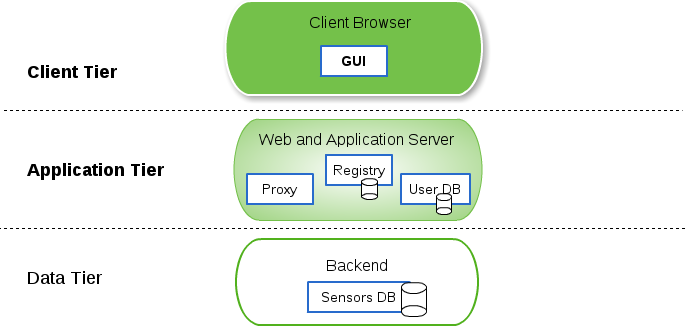
\includegraphics[scale=0.7]{images/3tier.png}   
  \caption[3-tier Architecture]{3-tier Architecture}
  \label{img:3-tier Architecture}                           
  \end{figure}

  \emph{Client Tier} hosts the presentation layer components. The main function of the interface is to translate tasks and results from application tier into a user-friendly GUI via client framework. This tier was defined in order to satisfy next requirements to the concept: cross-platform application, usability properties and responsiveness of a concept, which is formulated in the Section 2.1.

  \emph{Application Tier} includes business logic and data access tiers. It controls an application's functionality by performing detailed processing, transformation of a one type data to another, defines an interface of interconnection between client tier and data tier. Besides possessing application logic between two another tiers of infrastructure, this tier also consists integration point with a backend system. Loose coupling and multi-user binding discovered and implemented in this tier.

  \emph{Data Tier} consists source of data that have to be retrieved by application tier to a client tier, by request from a user. This tier keeps data neutral and independent from application server or business logic. Backend generates description of a data source in a defined by system way and provides access to the description and data itself through the standardized intreface.

   From a historical perspective the three-tier architecture concept emerged in the 1990s from observations of distributed systems\cite{wiki:3tier}(e.g., web applications) where the client, application and data tiers ran on physically separate platforms. Nowadays, MVC and similar model-view-presenter (MVP) are used as separation of concerns techniques. It discovers design patterns that apply exclusively to the presentation layer of a large system. In simple scenarios MVC may represent the primary design of a system, reaching directly into the database. Thus, to ensure highly adaptive GUI independently from a data and application tiers, MVC pattern come into a picture. As a part of frontend logic it will be described in the next subsection.
  
  The multi-tier architecture model may seem similar to the model-view-controller(MVC) concept. However, topologically they are different. A fundamental rule in a three tier architecture is the client tier never communicates directly with the data tier; in a three-tier model all communication must pass through the middle tier. Conceptually the three-tier architecture is linear. However, the MVC architecture is triangular: the view sends updates to the controller, the controller updates the model, and the view gets updated directly from the model.

  The next section describes every functional module of a respective tier according to 3-tier architecture.

\section{Client Tier}
  The client tier or another name is presentation tier is a layer which user can directly access from any type of portable device. In the Section 3.2 was proved necessity to implement web based portable application, which a user can access by using browser. This tier consists user-friendly GUI which includes widgets structured according to the responsive layout and client framework. First of all, client tier gives an overview of a design layout(Fig.\ref{img:GUI Mockup}), content provided by data source and managment panel(e.g. technical details of a system architecture such as: end-points configuration, API documentation or SDK downloads). Secondary, it contains client-based library to tire client tier with application tier. This tier also responsible for adaptation of a GUI to any kind of mobile or desktop devices. 
  \subsection{Web-based GUI Composition}

  Figure \ref{img:GUI Mockup} presents simple content layout that have to be presented on a web-page in order to satisfy all possible user requirements. It contains:

    \begin{figure}[!ht]
    \centering
    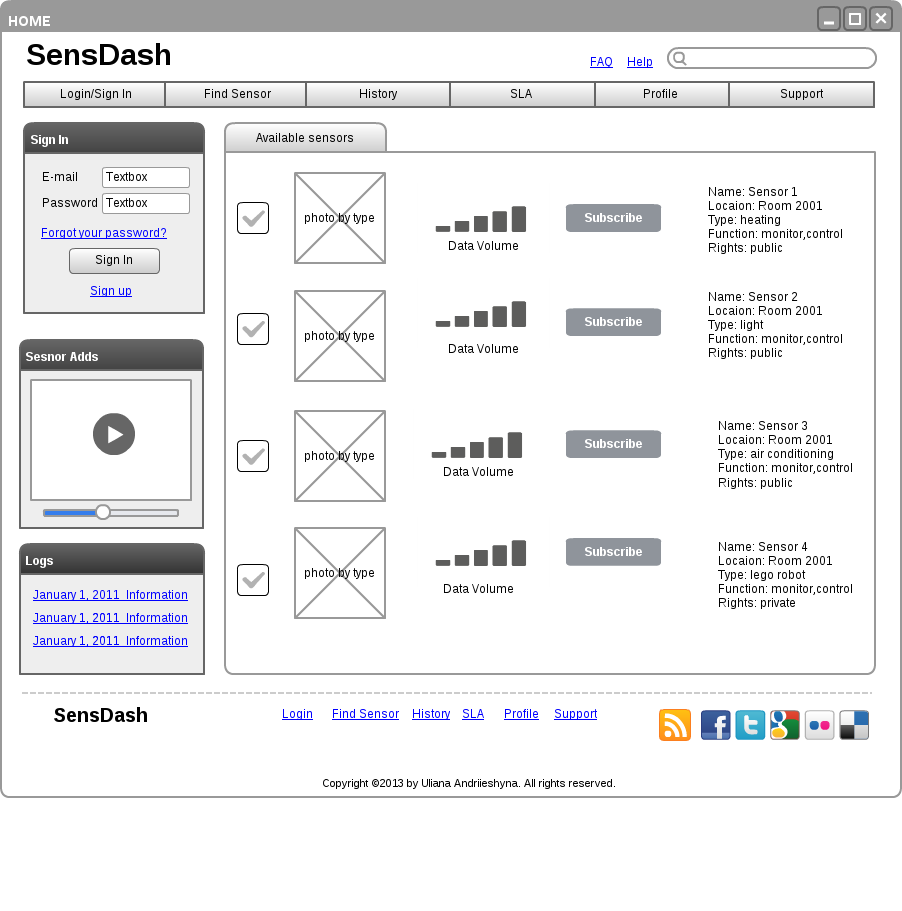
\includegraphics[scale=0.5]{images/Mockup.png}   
    \caption[GUI Mockup]{GUI Mockup}
    \label{img:GUI Mockup}                           
    \end{figure}

      \begin{itemize}
      \item Main five tabs: sensors list contains a list of all available sensors; subscriptions - show all data sources to which subscribed by a user; favorites tab saves favorite data sources among already subscribed; in the settings tab a user can manage own profile and also add new sensors by using corresponding form; and the admin references tab clarify steps needed to be established in order to develope own application.
      \item Log in form with user name and password. After user logged in, the system defines his/her rights and applies visibility rules according to assigned role. All users can explore description of every data retrieved by system, but only after subscription to a sensor become possible to get real-time streaming data. Users that have an admin rights receives an opportunity to manage sensors. Simple user without privileges, receives an opportunity to get statistic and information from sensors and to maintain his/her own account data.
      \item Sensor icon defines what is the current type of sensor, e.g. light, temperature, heating, robot lego battery status etc. It helps easily, even in seconds, understand and catch what is the main function of a sensor in the list, especially helpful wiil be to use famous vendor's icon.
      \item Availability or unavailability of a data source. User can subscribe only to the online services. If some services become offline it will be automatically marked as inactive and after refreshing of the page will be deleted from the list of available sensors. As soon as new data will be sended, a user will immendiatyely see it on the subscriptions tab. If user has already subscribed to any sensor, this sensor automatically added to a list/tab of subscriptions made by user. Also a user can define hierarchy in which sensor information have to be displayed. It is done by using ``favorite'' label/tab. It helps user to receive information from a sensor in a fast way.
      \item Data Volume icon shows the average data stream volume needed to retrieve sensor data(Kb/s). User can self-define how possible to get such type of streaming data according to his/her available Internet connection. Ideally, the dashboard should automatically adapt quality of streaming data based on connection throughput. Not only data volume depends on quality of a service itself, but also security level, reliability and performance. Such type of data description can be substituted by most relative icons such as: ``lock'' icon to define security level or appearance of a reliability label.
      \item Description and preview. The best way to give a user full information about data source is to provide a preview or examples of source data. It is not only description but also real-time drawing graphics, real example of video or audio, images etc.
      \item Access and providers. Based on provider of a data source, data can be private or public. For public type of data a user do not have to accept any SLA to subscribe to sensor. But for private data very important to accept SLA between subscriber and provider, before user will get any real data.
      \item Search panel. Need to filter and search between available sensors, which only based on information available for client tier. Without any queries to application or data tier.
      \end{itemize}

    The general use case shown on Figure \ref{img:use_case_basic}. User can use any type of mobile device and his favorite browser to receive information from data sources(sensors) by using web-page as a dashboard. Once a user log in to the dashboard, he/she can explore all available sensors. If he/she already a user of a dashboard all his/her preferences will be loaded from a server automatically and appear in respective tabs.

        \begin{figure}[!ht]
        \centering
        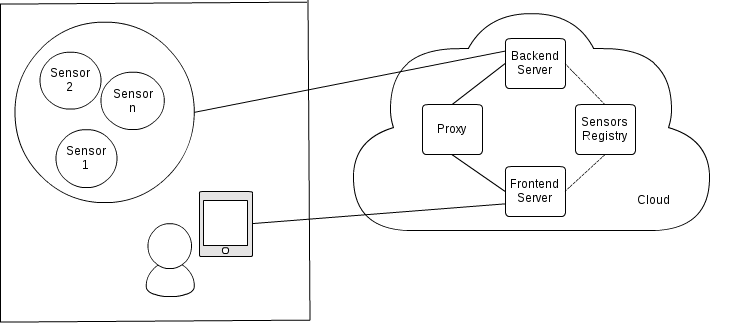
\includegraphics[scale=0.6]{images/User_Case.png}   
        \caption[Use Case]{Use Case}
        \label{img:use_case_basic}                        
        \end{figure}

    \subsection{JavaScript MVC}
    As was mentioned on the begining of section, the second responsibility of a client tier is to bind application and client tiers. It can be done by using client-based framework which is based on MVC pattern.

    In the design shown on the Figure \ref{img:MVCPattern}, takes place common Model-View-Controller pattern. Where a Model represents the application object that implements the application data and business logic. The View is responsible for formatting the application results and dynamic page construction. The Controller is responsible for receiving the client request, invoking the appropriate business logic, and based on the results, selecting the appropriate view to be presented to the user. The Model represents data and the business rules that govern access to and updates to this data. A View renders the contents of a Model. It accesses data through the Model and specifies how that data should be presented. It is the View's responsibility to maintain consistency in its presentation when the Model changes. This can be achieved by using a push Model, where the View registers itself with the Model for change notifications, or a pull Model, where the View is responsible for calling the Model when it needs to retrieve the most current data. A Controller translates interactions with the View into actions to be performed by the Model. In a stand-alone GUI client, user interactions could be button clicks or menu selections, whereas in a Web application, they appear as GET request. The actions performed by the Model include activating business processes or changing the state of the Model. Based on the user interactions and the outcome of the Model actions, the Controller responds by selecting an appropriate View.

    %  JavaScript has become one of the most popular programming languages on the web, when the usage of Ajax came to light and professional programmers gave importance to the responsiveness of the page. But now the language has become more popular than ever as the user experience has become the key part of web development. Accessing web is not limited to browsers alone – there are lot many devices with varying screen sizes accessing the same content. With the rise of HTML5 and CSS3 the web will become more adaptive and responsive than ever and JavaScript plays a major role in it. It has also gained popularity in the server side programming which is made possible by NodeJS framework.

    %Increased usage of JavaScript in modern applications has led to write maintainable code, separate concerns and improve testability. JavaScript is a "class"-less language and it was not designed to support Object Oriented Programming. There are some DOM manipulation libraries like jQuery which simplifies client side scripting of HTML, they actually do not solve the problem of effectively handling separation of concerns. The problem with this is that it doesn't take long to get lost in a nested pile of jQuery callbacks and DOM elements without any real structure in place for applications. Source code that has a complex and tangled control structure, especially one using many GOTOs, exceptions, threads, or other "unstructured" branching constructs can lead to become a bottleneck. 
     \begin{figure}[!ht]
     \centering
     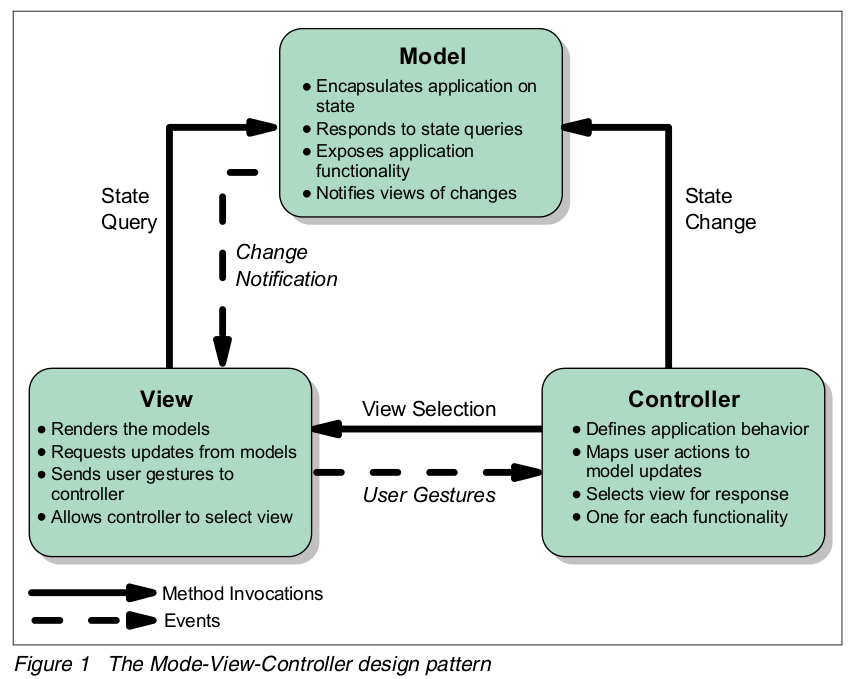
\includegraphics[scale=0.5]{images/MVCPattern.png}   
     \caption[MVC Pattern]{MVC Pattern\footnotetext{Image taken from, \url{blog.csdn.net/cain/article/details/6617173}}}
     \label{img:MVCPattern}                           
     \end{figure}
  
  Not necessary to follow the MVC pattern strictly. The idea of all the patterns is to separate Model, View and Logic that hooks the two behind which is the controller for the best separate of concerns.

\section{Application Tier}
  This layer coordinates processes commands, makes logical decisions and performs calculations. It also moves and processes data between the two surrounding layers.

  Application tier consists all logical modules: Web server, Registry, Data Hub and Web-based Frontend. All these modules connect to each other as shown on the Figure \ref{img:structure}. 
    \begin{figure}[!ht]
    \centering
    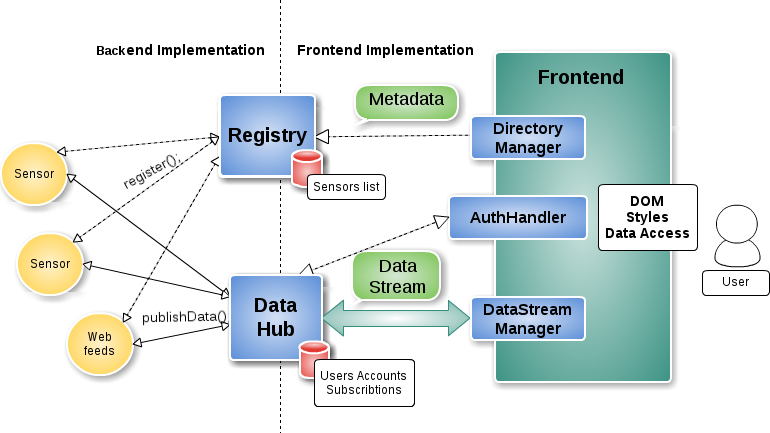
\includegraphics[scale=0.6]{images/Structure.png}   
    \caption[System Architecture]{System Architecture} 
    \label{img:structure}                        
    \end{figure}

    System Architecture splitted to a backend and frontend, that gives an overview of how these two parts interconnected. Respectively ``backend/frontend implementation'' means that all modules of each side have to be implemented separately. Such module as Registry and Data Hub defined and standardized by frontend, in order to clarify interface of collaboration with backend. To the backend responsibility relate an implementation of Registry and Data Hub modules.

  \subsection{Registry}
    The Registry is a module responsible for storing an info about all registered sensors in order to provide descriptional overview to a user. Frontend's GUI requests and aggregates info from Registry about registered in it data sources and dynamically presents it to the user. Registry contains next necessary attributes: unique id of a sensor, title, description, availability(true or false), access(private or public), provider of sensed data, SLA and its last update time, number of end-points available for one sensor and data format. JSON format fully satisfies described metadata format. The type of connection interface between Registry and Frontend will be defined in the Section 4.3.3. Defined structure of sensors' attributes within JSON format, describes sensors metadata and gives an opportunity to transform it automatically to the graphical container of a GUI. Registries which provides defined standard can be easily added to the frontend in a runtime. The Registry specifies simple interface standard in JSON format to encode all available attributes and properties and it is much simpler and light-weighted than XML and separate metadata of a sensor from a real-time data stream. 

    Before publishing data to Registry, a data publisher, which is a part of backend, have to fill in all attributes based on a description of a sensor. An important attribute of a sensor is its ``id''. It must be unique for every data source, in order to avoid inconsistency between different Registries. End-points for a sensor, handles real-time data streaming and have to be sctuctured in heuristic order, in order to switch between end-points when another one is failover. The number of end-points through which data streaming are performed not limited.

  \subsection{Data Hub}
    Since the Registry responsible for collecting metadata of sensors, Data Hub is responsible for mapping interface of particular sensor data stream format into a format supported by frontend and delivered through the common universal protocol. It means that Data Hub has to satisfy next requirements:

    \begin{itemize}
    \item be aware of metadata provided by Registry to frontend;
    \item bind metadata from Registry with real-time data streaming from sensor;
    \item get and parse sensor streaming data and reconvert it to the type supported by universal protocol;
    \item implement universal protocol to provide exchange message with a server in order to retrieve streaming data from sensor;
    \item store history from a sensors and user personal preferences.
    \end{itemize}
    
    A GUI depends a lot on user personal preferences. It may consist sensor subscriptions list, favorite data sources, user profile and list of available sensors. All these data have to be stored on the Data Hub and loaded after authentication process was sucessfully passed.

  \subsection{Web-based Frontend}
  \label{section:web-frontend}
    \subsubsection{Web server}
    The primary function of a web server is to deliver web pages to clients. The communication between client and server takes place using the Hypertext Transfer Protocol (HTTP). Pages delivered are most frequently HTML documents, which may include images, style sheets and scripts in addition to a text content. 
  
    In proposed concept Web server is responsible for robust and efficient serving of static files(*.html, *.css, *.js etc.). The goal is to exclude dependencies on concrete backend platforms or frameworks and to provide generic frontend as easily plugable component. Such a common and simplified design makes possible to extend and scale every part of a distributed system independently. Specific operation logic like authentication of user, registration of sensors and users are delegated to external components such as Registry, Data Hub and Authentication Hadler(AuthHandler), these external components can be interchanged without dependency to the system itself.

    \subsubsection{AuthHandler}
    Authentication Handler(AuthHandler) responsible for registering and log in a user to the the system. After a user gets necessary ID and confirm his/her personality by using password and name, system automatically applies visibility rules. After verification and confirmation of credentials, stored on a Data Hub, it becomes possible to bind user ID with personal preferences. These preferences include: user subscriptions, favorites, social sharing information and cookies.

    \subsubsection{Interfaces}
      On the Figure \ref{img:structure} exist 3 communication channels: 
      \begin{itemize}
      \item Registry to Directory Manager (one-way connection);
      \item Data Hub to/from DataStream Handler (asynchronous duplex connection);
      \item Data Hub to/from AuthHandler (synchronous duplex connection). 
      \end{itemize}

      \textbf{Registry to Directory Manager Interface}
      \newline
      Registry contains pairs of attributes - values, which describe sensors. These type of data can be structured by using JSON format and retrieved by Directory Manager through one-direction channel via HTTP GET request. The Directory Manager sends HTTP GET request to the Registry in order to get list of availale sensors and their metadata. Once JSON file is parsed by frontend, values of attributes extracted and aggregated as graphical container with all dependencies. HTTP GET request and JSON format is a part of RESTful API approach. Combination of JSON fromat and HTTP GET request in the future sesctionas will be called Web API.

      If system needs to use more then one Registry, requests will be sent to all of them. After getting all JSON lists of sensors, frontend will reparse all received data foming a sensor list and immediately aggregate it on a web page.

      \textbf{Data Hub -- Directory Manager Interface/AuthHandler}
      \newline
      Communication between Data Hub and another 2 modules: DataStream Handler and AuthHandler, have to be supported through the one common universal interface. It has to satisfy next requirements:
      \begin{itemize}
      \item have a public license;
      \item handle HTTP request from browser;
      \item support multiple channels in one connection;
      \item transfer different types of data in one channel, message differentiation;
      \item keep connection alive(stateful, through the TCP in background);
      \item simplicity of enhancement and customization.
      \end{itemize}

      The Data Hub -- Directory Manager/AuthHandler Interface flow are shown on the Figure \ref{img:protocol}. Such architecture decouple sensor specific interface and interface between frontend and backend.

      \begin{figure}[!ht]
      \centering
      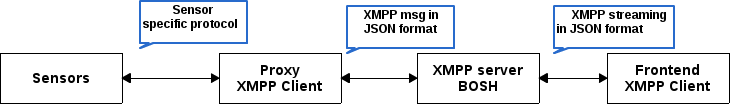
\includegraphics[scale=0.6]{images/Protocol_flow.png}   
      \caption[Protocol flow]{Protocol flow}
      \label{img:protocol}                           
      \end{figure}

      In order to satisfy all aforementioned requirements, nowadays exist two main protocols: \emph{XMPP\cite{XMPPbook}}:a protocol for connecting devices to people, a special case of the device-to-server pattern, since people are connected to the servers and \emph{MQTT\footnote{MQ Telemetry Transport, \url{http://mqtt.org/}}}: a protocol for collecting device data and sending it to servers. 

      \textbf{MQTT}
      \newline
      the Message Queue Telemetry Transport, targets device data collection (Fig. \ref{img:MQTT}\footnote{What is MQTT?, \url{https://www.ibm.com/developerworks/}}). As its name states, its main purpose is telemetry, or remote monitoring. Its goal is to collect data from many devices and transport that data to the IT infrastructure. It targets large networks of small devices that need to be monitored or controlled from the cloud.
      \begin{figure}[!ht]
      \centering
      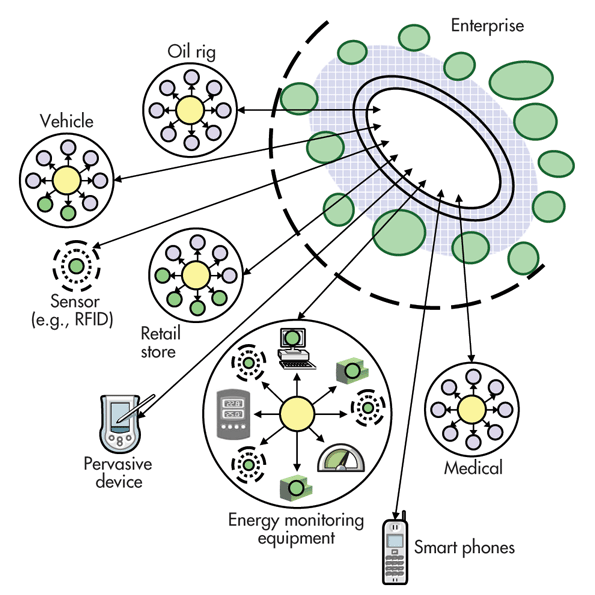
\includegraphics[scale=0.6]{images/MQTT.png}   
      \caption[Message Queue Telemetry Transport]{Message Queue Telemetry Transport}
      \label{img:MQTT}                           
      \end{figure}
      MQTT makes little attempt to enable device-to-device transfer, nor to ``fan out'' the data to many recipients. Since it has a clear, compelling single application, MQTT offering few control options. In this context, ``real time'' for MQTT is typically measured in seconds. All the devices connect to a data concentrator server. So the protocol works on top of TCP, which provides a simple, reliable stream. Since the IT infrastructure uses the data, the entire system is designed to transport data into enterprise technologies.

      MQTT enables applications like monitoring a huge oil pipeline for leaks or vandalism. Those thousands of sensors must be concentrated into a single location for analysis. When the system finds a problem, it can take action to correct that problem. Other applications for MQTT include power usage monitoring, lighting control, and even intelligent gardening. They share a need for collecting data from many sources and making it available to the IT infrastructure.

     \textbf{XMPP}
      \newline 
      XMPP was originally called ``Jabber''. It was developed for instant messaging (IM) to interconnect people via text messages (Fig. \ref{img:XMPP}\footnote{IoT, \url{http://electronicdesign.com/embedded/understanding-protocols-behind-internet-things}}). XMPP stands for Extensible Messaging and Presence Protocol. The targeted use is people-to-people communication.
      \begin{figure}[!ht]
      \centering
      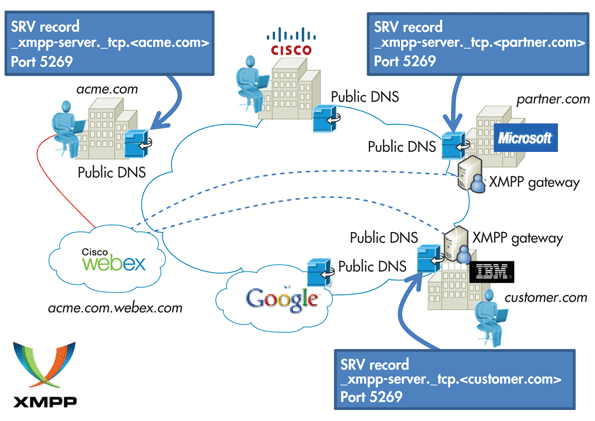
\includegraphics[scale=0.7]{images/XMPP.png}   
      \caption[The Extensible Messaging and Presence Protocol (XMPP)]{The Extensible Messaging and Presence Protocol (XMPP)}
      \label{img:XMPP}                           
      \end{figure}
      XMPP uses the XML text format as its native type, making person-to-person communications natural. Like MQTT, it runs over TCP, or over HTTP on top of TCP. Its key strength is a name@domain.com addressing scheme that helps connect the needles in the huge Internet haystack. XMPP powers a wide range of applications including instant messaging, multi-user chat, voice and video conferencing, collaborative spaces, real-time gaming, data synchronization, and even search. Although XMPP started its life as an open, standardized alternative to proprietary instant messaging systems like ICQ and AOL Instant Messenger, it has matured into an extremely robust protocol for all kinds of exciting creations.

      In fact, most implementations use polling, or checking for updates only on demand. A protocol called \emph{BOSH} (bidirectional streams over Synchronous HTTP) lets servers push new messages and ``real time'' to XMPP measured in seconds. The core of XMPP is the exchange of small, structured chunks of information. Like HTTP, XMPP is a client-server protocol, but it differs from HTTP by allowing either side to send data to the other asynchronously. XMPP connections are long lived, and data is pushed instead of pulled. Because of XMPP’s differences, it provides an 
      companion protocol to HTTP. XMPP also has nearly 200 extensions, providing a broad and useful range of tools on which to build sophisticated applications. 

      After a short introduction become clear that XMPP fully satisfy all requirements in order to be used in concept of a generic frontend. So the interface \emph{Data Hub to/from Directory Manager Interface/AuthHandler} provided by using XMPP. Thus, it should be discovered in details.
   
      XMPP, like all protocols, defines a format for moving data between two or more communicating entities. In XMPP’s case, the entities are normally a client and a server, although it also allows for peer-to-peer communication between two servers or two clients. Many XMPP servers exist on the Internet, accessible to all, and form a federated network of interconnected systems. Data exchanged over XMPP is in XML, giving the communication a rich, extensible structure. One major feature XMPP gets by using XML is XML's insensibility. This extensibility is put to great use in the more than 200 protocol extensions registered with the XMPP Standards Foundation and has provided developers with a rich set of tools. XML is known primarily as a document format, but in XMPP, XML data is organized as a pair of streams, one stream for each direction of communication. Each XML stream consists of an opening element, followed by XMPP stanzas and other top-level elements, and then a closing element. Each XMPP stanza is a first-level child element of the stream with all its descendant elements and attributes. At the end of an XMPP connection, the two streams form a pair of valid XML documents. The Extensible Messaging and Presence Protocol is the IETF's formalization of the base XML streaming protocols for instant messaging and presence developed within the Jabber community\cite{xmpp}.

      \textbf{Pushing Data}

      HTTP clients can only request data from a server. Unless the server is responding to a client request,
      it can not send data to the client. XMPP connections, on the other hand, are bidirectional. Either party
      can send data to the other at any time, as long as the connection is open. This ability to push data expands the possibilities for web applications and protocol design. Instead of inefficient polling for updates, applications can instead receive notifications when new information is available.

      \textbf{Pleasing Firewalls}

      Some web applications support the use of HTTP callbacks, where the web server makes requests to another HTTP server in order to send data. This would be a handy feature to push data if it were not for firewalls, network address translation (NAT), and other realities of the Internet. In practice it is very hard to enable arbitrary connections to clients from the outside world. XMPP connections are firewall and NAT friendly because the client initiates the connection on which server-to-client communication takes place. Once a connection is established, the server can push all the data it needs to the client, just as it can in the response to an HTTP request.
      
      \textbf{Improving Security}

      XMPP is built on top of Transport Layer Security(TLS) and Simple Authentication and Security Layer (SASL) technologies, which provide robust encryption and security for XMPP connections. Though HTTP uses Secure Sockets Layer (SSL), the HTTP authentication mechanisms did not see much implementation or use by developers. Instead, the Web is full of sites that have implemented their own authentication schemes, often badly.
      
      \textbf{Statefulness}

      HTTP is a stateless protocol; XMPP is stateful. Stateless protocols are easier to scale because each server does not need to know the entire state in order to serve a request. This drawback of XMPP is less onerous in practice because most non-trivial web applications make extensive use of cookies, backend databases, and many other forms of stored state. Many of the same tools used to scale HTTP-based applications can also be used to scale XMPP-based ones, although the number and diversity of such tools is more limited, due to XMPP’s younger age and lesser popularity.

      Main XMPP properties are:
    \begin{itemize}
      \item \emph{Decentralization}. The architecture of the XMPP network is similar to email; anyone can run their own XMPP server and there is no central master server.
     \item \emph{Open standards}. The Internet Engineering Task Force has formalized XMPP as an approved instant messaging and presence technology under the name of XMPP (the latest specifications are RFC 6120 and RFC 6121). No royalties are required to implement support of these specifications and their development is not tied to a single vendor.
      \item \emph{History}. XMPP technologies have been in use since 1999. Multiple implementations of the XMPP standards exist for clients, servers, components, and code libraries.
      \item \emph{Security}. XMPP servers can be isolated from the public XMPP network (e.g., on a company intranet), and strong security (via SASL and TLS) has been built into the core XMPP specifications.
      \item \emph{Flexibility}. Custom functionality can be built on top of XMPP; to maintain interoperability, common extensions are managed by the XMPP Standards Foundation. XMPP applications beyond IM include group chat, content syndication, collaboration tools, file sharing, gaming, remote systems control and monitoring of geolocation, cloud computing, VoIP and Identity services.
      \end{itemize}

      \begin{figure}[!ht]
      \centering
      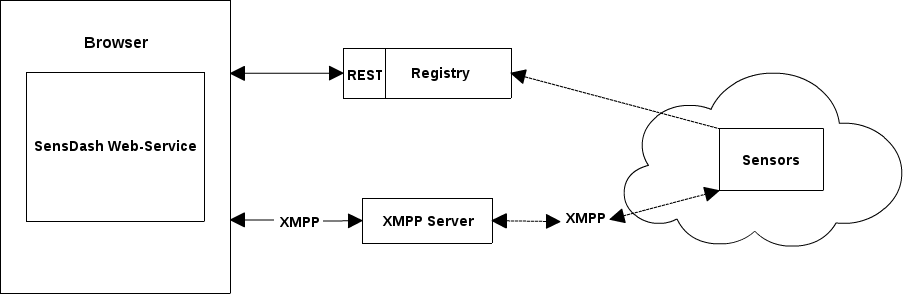
\includegraphics[scale=0.5]{images/Interface.png}   
      \caption[Interface]{Interface}
      \label{img:interfaces}                           
      \end{figure}

      The XMPP network uses a client-server architecture (clients do not talk directly to one another). However, it is decentralized by design, there is no central authoritative server. Anyone may run their own XMPP server on their own domain. Every user on the network has a unique Jabber ID (usually abbreviated as JID). To avoid requiring a central server to maintain a list of IDs, the JID is structured like an email address with a username and a domain name (or IP address) for the server where that user resides, separated by an at sign (@), such as username@example.com.  

\subsection{Backend Entry Points}
    Data Hub and Registry are two modules that have been standardized by frontend and have to be fully implemented on a backend side. Since both of these parts support common standards such as Web API, AJAX, JSON or XML file format, it makes possible to implement every functional module on a backend side without dependency on OS type, framework or language of implementation. Separation between metadata and streaming data increase scalaility of a system, such that any number of Registries and Data Hubs can be deployed in runtime. Defined Web API and XMPP-based interfaces between frontend's and backend's sides based on open standards. In case of XMPP-based interface, all communication are flows through a distributed XMPP network. Thus, Data Hub needs to have its own XMPP server or sends a requests through any alternative server.

\section{Data Tier}
   As was mentioned in the Section 4.1 data tier contains data sources that have to be retrieved via application tier to a client tier. Data tier consists of hardware and software sensors, which provide an information to a user. The data format which can be retrieved by frontend via XMPP connection has no limitation, but in scope of this master thesis was defined such type of information as text and map of values. Text format is used as an example of information provided by software sensor. In the same time hardware sensor periodically sends measured map o values. These types of data changes with some time-frequency and automatically retrieved by THE client tier as a real-time data stream.

  An important aspect in streaming data that some of data can be cashed on a server side, thus become possible to retrieve data after it was produced. But some streaming data consists only live data, thus there is no other options except live streaming, where the connection configuration, aliveness and quality become a key aspect. All these properties are already covered by XMPP. Consider absence of any concrete backend system, cashing of a data can be done based on XMPP server configuration. 

  \textbf{Sensor Functional Characteristics}
  \newline
  An essential part of a concept is to garantee reliable and secure data transportation. Thus, every data source can acquire additional properties based on a system architecture:
  \begin{itemize}
  \item reliability,
  \item perfomance,
  \item security.
  \end{itemize}
  All these three characteristics rely on a quantity of available Data Hubs which include XMPP modules and handle data streaming. Since Data Hub have to provide data from a sensor to a frontend by using XMPP connection, it has to support XMPP data channel configurations and may play a role of end-point for frontend. If sensor has 2 end-points it should be mentioned in Registry together with a type of data transfer protocol(covered in the Section 5.2).

  A simple sensor, with a low level of reliability, has one and only one end-point(Figure \ref{img:end_points} a). A reliable sensor has two end-points, where is one is a primary, the other one is a backup/failover(Figure \ref{img:end_points} c). A highly reliable sensor has three end-points, which is guarantee data arrival in case of failover of another end-points. 
     \begin{figure}[!ht]
     \centering
     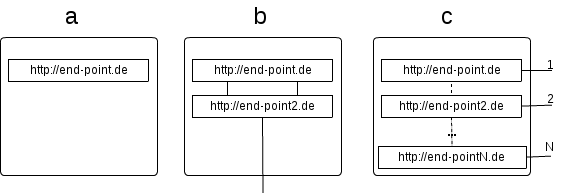
\includegraphics[scale=0.6]{images/FuncCharacteristics.png}   
     \caption[MVC Pattern]{Sensor Functional Characteristics} 
     \label{img:end_points}                     
     \end{figure}
  A high-performance sensor has more than 2 end-points(Figure \ref{img:end_points} c), out of which one is always chosen based on minimal latency message income. In case of big data transportation, all data can be splitted and partially  sended in parallel through more than 2 end-points. 
    
  A secure sensor maintained by at least two end-points, each of which carries some part of a data(Figure \ref{img:end_points} b). Without each part of a message become not possible to retrieve whole data at all. 

 All functional characteristics have to be automatically captured by frontend from a predefined attributes located in a Registry. So that user can get to know about the expected quality of the data streams even in case some end-points become unavailable. In the meanwhile, frontend has predefined logic, which calculates numbers of related end-point for every sensor and by using graphical elements such as icons and labels, presents this information to the user on the welcome screen. In case of failover of an end-point and data source has additional end-point, frontend automatically  reconnects to the next end-point, by using AJAX request, and user can continue receiving data. Such users, as developer of a mobile application, which wants to use frontend as a proxy for their application, would be necessary to understand the order of end-points, and clarify how to interconnect them in order to provide high-secure, reliable and high-performance data retrieval.

\section{Summary}
	In this chapter, according to a 3-tier architecture, the first web-based concept for sensor streaming services is to be created. Fine-grained structure provides clear separation of concerns between different module of concept. Client tier consists GUI content and client framework; Application tier provides application logic in order to interconnect backend and Client tier; and finally, Data tier describes typization of data in order to interconnect it  easily  with Application tier and visually retrieve it by using Client tier. To an every data souce was assigned such functional characteristics as reliability, perfomance and security level of information. Every characteristics rely on a number of responsible for sensor end-points. 

    As a result fine-grained structure of a concept was built on top of next modules: 
 Registry responsibilities:
  \begin{itemize}
  \item stores an metadta about available sensors registered in the network;
  \item provides Web API by using JSON format.
  \end{itemize}
  Data Hub responsibilities:
  \begin{itemize}
    \item be aware of metadata provided by Registry to a frontend;
    \item bind metadata from Registry with real-time data streaming from sensor;
    \item get and parse sensor streaming data and reconvert sensor-specific protocol to a XMPP;
    \item implement XMPP services and quarantee message exchenge between frontend and sensors;
    \item store history of a data sources and personal user preferences.
  \end{itemize}

  Web-server responsibilities: handles delivery to a user static structure of the web-page.

  Frontend responsibilities:
  \begin{itemize}
  \item interconnect all modules by using appropriate interfaces: Web API for Registry and XMPP interface for Data Hub and AuthHandler;
  \item build a responsive and adaptive to changes GUI;
  \item scalable system structure(Adding new Registries through Web form, changing personal preferences).
  \end{itemize}